\documentclass[11pt]{amsart}
\usepackage{amsmath,amssymb,stmaryrd}
\setlength{\emergencystretch}{3em}
\tolerance=600
\usepackage{tikz}
\usetikzlibrary{arrows.meta,decorations.pathreplacing}
\usepackage{tikz-cd}
\usepackage[hidelinks]{hyperref}

\newtheorem{thm}{Theorem}[section]
\newtheorem{lem}[thm]{Lemma}
\newtheorem{cor}[thm]{Corollary}
\newtheorem{prop}[thm]{Proposition}
\theoremstyle{definition}
\newtheorem{defi}[thm]{Definition}
\newtheorem{rem}[thm]{Remark}
\newtheorem{ex}[thm]{Example}
\newtheorem{que}[thm]{Question}

\newcommand{\Fix}{\mathrm{Fix}}
\newcommand{\Up}{\mathrm{Up}}
\newcommand{\Nuc}{\mathrm{N}}
\newcommand{\Same}{\mathrm{Same}}
\newcommand{\FSet}{\mathbf{Set}}
\newcommand{\Bij}{\mathrm{Bij}}
\newcommand{\LLJ}{\mathbf{LJ}}
\newcommand{\lax}{\bigcirc}
\newcommand{\laxa}{\bigcirc_1}
\newcommand{\laxb}{\bigcirc_2}
\newcommand{\sL}{\mathsf{L}}

\begin{document}

\title[Nuclei and the sameness lattice of fuzzy sets]{Nuclei on the algebra of truth values and the sameness lattice of fuzzy sets: meets, joins and the finite-iteration axiom}
\author{Ryota Shibusawa}
\thanks{Corresponding author. E-mail: \texttt{r-shibusawa@daiichi-koudai.ac.jp}}
\address{Daiichi Institute of Technology}
\email{r-shibusawa@daiichi-koudai.ac.jp}
\keywords{fuzzy set, residuated lattice, nucleus, closure operator, MV-algebra, G\"odel algebra,
  reflective subcategory, two-out-of-three, lax logic}
\subjclass[2020]{03E72 (primary), 06F05, 18A40, 03B52, 03B45 (secondary)}

\begin{abstract}
Let $L$ be a complete residuated lattice of truth values and $\FSet(L)$ the
category of $L$-fuzzy sets. A nucleus $j$ on $L$, a closure operator with
$ja\otimes jb\le j(a\otimes b)$, determines the reflective subcategory of
$j$-closed fuzzy sets, with reflector $(X,\mu)\mapsto(X,j\mu)$, and hence the
class $W_j$ of maps inverted by the reflector, the isomorphisms up to $j$;
these classes are elements of the lattice $\Same(\FSet(L))$ of classes of
maps closed under composition and two-out-of-three. We show that
$j\mapsto W_j$ is an injective map from the lattice of nuclei preserving all
meets, and that it preserves the join of two nuclei $j_1,j_2$ exactly when
the alternating iterate $(j_2j_1)^N$ equals $j_1\vee j_2$ for some $N$, the
finite-iteration axiom of the lax logic of the join; in the lattice
$\Same(L)$ of the poset $L$ itself, pointwise stabilisation suffices. On a
complete MV-algebra every nucleus is closed, $ja=a\vee c$, and on the
product chain every nucleus is a closed nucleus or its restriction to the
positive degrees; in both cases the alternating iteration stabilises in two
steps, and the lattice of nuclei embeds as a lattice into the sameness
lattice of fuzzy sets, for MV-algebras as the algebra of truth values
itself; the lax modality of \L ukasiewicz logic is a disjunction with a
constant. On the G\"odel chain $[0,1]$ nuclei are arbitrary inf-closed
subsets, and we give pairs for which the join is preserved in $\Same(L)$ but
not in $\Same(\FSet(L))$, and pairs for which it is preserved in neither.
\end{abstract}

\maketitle

\section{Introduction}

Fuzzy set theory takes its truth values in a complete residuated lattice $L$
\cite{Goguen,Hajek}: a fuzzy set is a map $\mu\colon X\to L$, and a map of
fuzzy sets $(X,\mu)\to(Y,\nu)$ is a function $f$ with $\mu\le\nu\circ f$. The
resulting category $\FSet(L)$ of Goguen \cite{Goguen} is the setting of this
paper. The second ingredient is a \emph{nucleus} on $L$, a closure operator
$j$ with $ja\otimes jb\le j(a\otimes b)$ \cite{Rosenthal,GJKO}. When $L$ is a
frame, nuclei are the Lawvere--Tierney topologies of the topos of sheaves on
$L$ and the sublocales of $L$ \cite{Johnstone}; in general they are the
quotients of $L$ as a residuated lattice and the semantics of the lax
modality of intuitionistic and substructural modal logic
\cite{FM,Laxjoin}. A nucleus acts on fuzzy sets degreewise: $(X,\mu)\mapsto
(X,j\mu)$ is the reflection of $\FSet(L)$ onto the full subcategory of
$j$-closed fuzzy sets, those with $\mu=j\mu$, and the reflection sends a map
$f$ to an isomorphism exactly when $f$ is a bijection with $j\mu=j\nu\circ f$:
the fuzzy sets agree once their degrees are rounded up by $j$. We write $W_j$
for this class of maps, the \emph{isomorphisms up to $j$}.

The classes $W_j$ live in the lattice $\Same(\FSet(L))$ of \emph{samenesses}
of $\FSet(L)$, the classes of maps containing the identities and closed under
composition and two-out-of-three, studied in \cite{Same,Topjoin,Finitejoin,
Varieties} for Grothendieck topologies and for subvarieties. The question of
those papers is how the lattice operations of the indexing structure, here
the lattice $\Nuc(L)$ of nuclei, are reflected in $\Same$. The answer here is
complete.

\begin{thm}\label{thm:main}
Let $L$ be a complete residuated lattice.
\begin{enumerate}
\item[(i)] $j\mapsto W_j$ is an injective, order-preserving map
$\Nuc(L)\to\Same(\FSet(L))$ that preserves all meets:
$W_{\bigwedge_ij_i}=\bigcap_iW_{j_i}$ for every family of nuclei.
\item[(ii)] For nuclei $j_1,j_2$ preserving binary meets,
$W_{j_1\vee j_2}=W_{j_1}\vee W_{j_2}$ if and only if there is $N$ with
$(j_2j_1)^N=j_1\vee j_2$.
\end{enumerate}
The same holds for the classes $W_j^L=\{a\le b:\ ja=jb\}$ in the sameness
lattice $\Same(L)$ of the poset $L$, except that in (ii) the condition is
pointwise: for every $a\in L$ some iterate $(j_2j_1)^na$ equals $(j_1\vee j_2)a$.
\end{thm}

Every nucleus on a Heyting algebra, every nucleus on an MV-algebra and every
closed nucleus $a\mapsto a\vee c$ on a distributive lattice preserves binary
meets, so (ii) covers the standard algebras of fuzzy logic. The condition in
(ii) is the \emph{finite-iteration axiom} $(\laxb\laxa)^N\varphi\leftrightarrow
\lax\varphi$ of the trimodal lax logic $\LLJ$ of two nuclei and their join
\cite{Laxjoin}, valid on every finite algebra and on $\Up(P)$ for finite
posets $P$ with $N=|P|$; Theorem~\ref{thm:main} says that this axiom is
exactly what makes the join of two nuclei visible at the level of
isomorphisms of fuzzy sets. The gap between the pointwise and the uniform
condition separates $\Same(L)$ from $\Same(\FSet(L))$.

For the standard algebras the picture is as follows (Section~\ref{sec:std}).
On a complete MV-algebra $A$, in particular on the \L ukasiewicz chain
$[0,1]$, every nucleus is closed, $ja=a\vee c$: the fixed points of a
nucleus are closed under $a\to b$, and $\{a\to b:a\in A\}$ is the whole
principal filter $\uparrow\!b$. Hence $\Nuc(A)\cong A$, two alternating
steps always suffice, and $c\mapsto W_{a\mapsto a\vee c}$ is a lattice
embedding $A\hookrightarrow\Same(\FSet(A))$: the algebra of truth values is a
sublattice of the sameness lattice of its fuzzy sets, $W_c$ being the class
of bijections under which the two fuzzy sets agree above the threshold $c$.
On the product chain $[0,1]_\Pi$ the residual $a\to0$ takes only the values
$0$ and $1$, and besides the closed nuclei there are their restrictions to
the positive degrees, $q_c(a)=a\vee c$ for $a>0$ and $q_c(0)=0$; still two
alternating steps suffice and $\Nuc([0,1]_\Pi)$ embeds as a lattice. On the G\"odel chain $[0,1]$, by
contrast, a nucleus is any inf-closed set of fixed points containing $1$, and
we give two nuclei whose alternating iteration stabilises at every point but
not uniformly, so that the join is preserved in $\Same(L)$ and not in
$\Same(\FSet(L))$, and two nuclei for which it is preserved in neither.

\subsection*{What is known.}
Nuclei on frames, quantales and residuated lattices and their lattice are
classical \cite{Johnstone,Rosenthal,GJKO}; the join of two nuclei is the
least common fixed point operator, reached by transfinite iteration of the
composite \cite{Macnab,Escardo}. Goguen's category of $L$-fuzzy sets is from
\cite{Goguen}; its relation to sheaves on a frame is due to Barr
\cite{Barr}. Samenesses and the behaviour of meets and joins of Grothendieck
topologies and of subvarieties in $\Same$ are from
\cite{Same,Topjoin,Finitejoin,Varieties}, and the lax logic $\LLJ$ of the
join of two nuclei, with its finite-iteration axiom, from \cite{Laxjoin}.
Nuclei on residuated lattices are studied in \cite{GJKO}, and a
description of arbitrary nuclei on residuated lattices, with the terms that
define them on subvarieties of BL-algebras, is given by Buss, Casta\~no and
D\'\i az Varela \cite{BCD}. That nuclei on MV-algebras are closed is
elementary and may be known; we include the short proof, and we classify
the nuclei on the product chain.

\subsection*{What is new.}
Theorem~\ref{thm:main}: the meet-embedding $\Nuc(L)\hookrightarrow
\Same(\FSet(L))$ and the characterisation of the preservation of binary
joins by the finite-iteration axiom, with the pointwise variant for
$\Same(L)$; the description of $\Same(\FSet(L))$-joins by uniformly bounded
alternating chains (Lemma~\ref{lem:chains}); and the consequences for the
standard algebras, the lattice embeddings of $\Nuc(A)$ for complete
MV-algebras and for the product chain and the two G\"odel examples
(Section~\ref{sec:std}); the classification of nuclei on MV-algebras and on
the product chain is elementary.

\section{Fuzzy sets, nuclei and isomorphisms up to a nucleus}\label{sec:prelim}

Throughout, $L$ is a complete integral commutative residuated lattice: a
complete lattice with a commutative monoid operation $\otimes$ with unit
$\top$, distributing over arbitrary joins, and residual $\to$ with
$a\otimes b\le c$ iff $a\le b\to c$. Frames ($\otimes=\wedge$, G\"odel
logic), MV-algebras (\L ukasiewicz logic) and the product chain are
examples \cite{Hajek}.

\begin{defi}
A \emph{nucleus} on $L$ is a map $j\colon L\to L$ with $a\le ja$,
$jja=ja$, $a\le b\Rightarrow ja\le jb$ and $ja\otimes jb\le j(a\otimes b)$.
Its fixed points $\Fix(j)=\{a:ja=a\}$ are closed under arbitrary meets and
under $a\to b$ for $b\in\Fix(j)$; conversely every subset $F\subseteq L$
closed under meets and under $a\to(-)$ is $\Fix(j_F)$ for the nucleus
$j_F(a)=\bigwedge\{f\in F:f\ge a\}$ \cite{Rosenthal,GJKO}. Nuclei are
ordered pointwise; $\Nuc(L)$ is a complete lattice with pointwise meets,
$j\le k$ iff $\Fix(k)\subseteq\Fix(j)$, and the join $j_1\vee j_2$ is the
nucleus with $\Fix(j_1\vee j_2)=\Fix(j_1)\cap\Fix(j_2)$, i.e.\
$(j_1\vee j_2)(a)$ is the least common fixed point above $a$, the stable
value of the transfinite iteration $a\le j_1a\le j_2j_1a\le\cdots$
\cite{Macnab,Escardo}. A nucleus \emph{preserves binary meets} if
$j(a\wedge b)=ja\wedge jb$; this holds for every nucleus on a frame, where it
is part of the definition, and for closed nuclei $c_u(a)=a\vee u$ on
distributive lattices. A closure operator always satisfies
$j(a\vee b)=j(ja\vee jb)$.
\end{defi}

\begin{defi}
$\FSet(L)$ has as objects the pairs $(X,\mu)$ with $X$ a set and
$\mu\colon X\to L$, and as morphisms $(X,\mu)\to(Y,\nu)$ the functions
$f\colon X\to Y$ with $\mu(x)\le\nu(f(x))$ for all $x$. An isomorphism is a
bijection with $\mu=\nu\circ f$. For a nucleus $j$, a fuzzy set is
\emph{$j$-closed} if $\mu=j\mu$, and $\FSet_j(L)$ is the full subcategory
of $j$-closed fuzzy sets.
\end{defi}

\begin{lem}\label{lem:refl}
$\FSet_j(L)$ is reflective in $\FSet(L)$ with reflector $(X,\mu)\mapsto
(X,j\mu)$ and unit the identity function. The reflector inverts a map
$f\colon(X,\mu)\to(Y,\nu)$ if and only if $f$ is a bijection and
$j\mu=j\nu\circ f$. $\FSet_{j_1}(L)\cap\FSet_{j_2}(L)=\FSet_{j_1\vee j_2}(L)$,
and $j\le k$ iff $\FSet_k(L)\subseteq\FSet_j(L)$.
\end{lem}
\begin{proof}
If $(Z,\zeta)$ is $j$-closed and $f\colon(X,\mu)\to(Z,\zeta)$, then
$j\mu\le j(\zeta\circ f)=\zeta\circ f$, so $f$ is a map $(X,j\mu)\to(Z,\zeta)$,
uniquely through the unit. The reflector sends $f$ to the same function
regarded as $(X,j\mu)\to(Y,j\nu)$, which is an isomorphism iff $f$ is
bijective and $j\mu=j\nu\circ f$. A fuzzy set is closed under $j_1$ and
$j_2$ iff its degrees are common fixed points, i.e.\ fixed by
$j_1\vee j_2$. If $j\le k$ then $k\mu=\mu$ implies $j\mu\le k\mu=\mu$; if
$\FSet_k\subseteq\FSet_j$ then every $k$-fixed element is $j$-fixed, so
$j\le k$.
\end{proof}

\begin{defi}
For a category $C$, $\Same(C)$ is the complete lattice of classes of
morphisms containing all identities and closed under composition and
two-out-of-three (if two of $f$, $g$, $g\circ f$ are in the class, so is the
third), ordered by inclusion; meets are intersections and the join of two
classes is the least class containing both \cite{Same}. For a nucleus $j$
let
\[
W_j=\{f\colon(X,\mu)\to(Y,\nu)\text{ bijective with }j\mu=j\nu\circ f\}\in\Same(\FSet(L)),
\]
the class inverted by the reflector of Lemma~\ref{lem:refl}, which is a
sameness because classes inverted by a functor are. In the poset $L$,
viewed as a category with an arrow $a\to b$ for $a\le b$, let
$W_j^L=\{(a\le b):\ ja=jb\}\in\Same(L)$, the class inverted by the monotone
map $j\colon L\to L$.
\end{defi}

The class $\Bij$ of maps of fuzzy sets that are bijective on underlying
sets is a sameness, and $W_j\subseteq\Bij$. A bijective map is, up to
composition with isomorphisms, an identity function $(X,\mu)\to(X,\nu)$
with $\mu\le\nu$ pointwise; since isomorphisms belong to every sameness and
samenesses are closed under composition and cancellation with them,
membership of a bijection in a sameness depends only on the family of
pairs $(\mu(x)\le\nu(f(x)))_{x\in X}$. In this sense the whole discussion is
pointwise in $L$, and the only global feature is uniformity over $X$.

\section{Meets}\label{sec:meets}

\begin{thm}\label{thm:meets}
For any family $(j_i)_{i\in I}$ of closure operators on $L$ with pointwise
meet $j=\bigwedge_ij_i$,
\[
W_j=\bigcap_iW_{j_i}\quad\text{in }\Same(\FSet(L)),\qquad
W^L_j=\bigcap_iW^L_{j_i}\quad\text{in }\Same(L).
\]
Moreover $j\mapsto W_j$ and $j\mapsto W^L_j$ are injective and order-preserving.
Hence both are embeddings of complete meet-semilattices.
\end{thm}
\begin{proof}
If $j\le k$ then $kj=k$, so $j\mu=j\nu f$ gives $k\mu=kj\mu=kj\nu f=k\nu f$:
$W_j\subseteq W_k$. Injectivity: the pair $(a\le ja)$ lies in $W^L_j$, and in
$W^L_k$ iff $ka=kja$, i.e.\ $ja\le ka$; so $W^L_j=W^L_k$ forces $j=k$, and
the same pairs realised on one-point fuzzy sets give injectivity of
$j\mapsto W_j$. For the meets, $\supseteq$ is monotonicity. Conversely let
$f\colon(X,\mu)\to(Y,\nu)$ be a bijection with $j\mu=j\nu f$ and fix $x$,
$a=\mu(x)\le b=\nu(f(x))$. Then
\[
b\le jb=\textstyle\bigwedge_ij_ib=\bigwedge_ij_ia\le j_ka
\]
for every $k$, so $j_kb\le j_kj_ka=j_ka\le j_kb$. Hence $j_k\mu=j_k\nu f$
for all $k$. The argument for $\Same(L)$ is the case of one point.
\end{proof}

Theorem~\ref{thm:meets} uses nothing about $\otimes$: it holds for all
closure operators on a complete lattice. The pointwise meet of nuclei is
their meet in $\Nuc(L)$, so the theorem is statement (i) of
Theorem~\ref{thm:main}.

\section{Joins}\label{sec:joins}

Fix two nuclei $j_1,j_2$ on $L$ preserving binary meets, and write
$j=j_1\vee j_2$. An \emph{alternating chain} from $a$ to $b$ is a sequence
$a=c_0\le c_1\le\dots\le c_n=b$ together with indices
$p(1),\dots,p(n)\in\{1,2\}$ such that $j_{p(i)}c_{i-1}=j_{p(i)}c_i$ for all
$i$; its length is $n$. Repeating an element is a step of either index, so
chains can be padded, and the indices can be assumed to alternate
$1,2,1,2,\dots$ by inserting trivial steps; we do so.

\begin{lem}\label{lem:chains}
\begin{enumerate}
\item[(i)] $W^L_{j_1}\vee W^L_{j_2}$ in $\Same(L)$ is the set of pairs $a\le b$
joined by an alternating chain.
\item[(ii)] $W_{j_1}\vee W_{j_2}$ in $\Same(\FSet(L))$ is the set of bijections
$f\colon(X,\mu)\to(Y,\nu)$ for which there is $N$ such that every pair
$\mu(x)\le\nu(f(x))$ is joined by an alternating chain of length at most $N$.
\end{enumerate}
\end{lem}
\begin{proof}
Let $\mathcal U$ be the class in (ii); $\mathcal U\supseteq W_{j_1}\cup W_{j_2}$
(chains of length $1$) and $\mathcal U$ contains the identities. Each
element of $\mathcal U$ is a composite of elements of $W_{j_1}\cup W_{j_2}$:
given uniform chains $(c_i(x))_{i\le N}$ with alternating indices, the
identity functions $(X,c_{i-1})\to(X,c_i)$ lie in $W_{j_{p(i)}}$, and
$f$ is the composite of these with the isomorphism $(X,\nu f)\to(Y,\nu)$.
So it remains to show that $\mathcal U$ is a sameness. Composition
concatenates chains, with lengths adding. For cancellation let
$f\colon(X,\mu)\to(Y,\nu)$ and $g\colon(Y,\nu)\to(Z,\rho)$ with
$gf\in\mathcal U$; both are bijections if one of $f,g$ is in $\mathcal U$,
as $\Bij$ is a sameness. Fix $x$ and put $a=\mu(x)\le b=\nu(fx)\le c=\rho(gfx)$,
with a chain $a=c_0\le\dots\le c_n=c$ of length at most $N$.
If $g\in\mathcal U$ we need a bounded chain from $a$ to $b$:
$a=c_0\wedge b\le c_1\wedge b\le\dots\le c_n\wedge b=b$ is one, because
$j_{p(i)}(c_{i-1}\wedge b)=j_{p(i)}c_{i-1}\wedge j_{p(i)}b=j_{p(i)}c_i\wedge
j_{p(i)}b=j_{p(i)}(c_i\wedge b)$ by preservation of binary meets. If
$f\in\mathcal U$ we need a bounded chain from $b$ to $c$:
$b=c_0\vee b\le c_1\vee b\le\dots\le c_n\vee b=c$ is one, because
$j(c_{i-1}\vee b)=j(jc_{i-1}\vee jb)=j(jc_i\vee jb)=j(c_i\vee b)$ for
$j=j_{p(i)}$, using $j(u\vee v)=j(ju\vee jv)$. Both constructions preserve
the length, hence the uniform bound. This proves (ii), and (i) is the same
argument on one point, where no bound is needed.
\end{proof}

\begin{rem}
Preservation of binary meets is used only in the left cancellation, and
cannot simply be dropped from Lemma~\ref{lem:chains} for closure operators
in general. On the four-element Boolean lattice $\{0,a,b,1\}$ let $j_1$ fix
$0,a,1$ and send $b$ to $1$, and let $j_2$ fix $b,1$ and send $0$ to $b$
and $a$ to $1$; $j_1$ does not preserve $a\wedge b$. The pairs $(0\le b)$,
$(b\le1)$, $(a\le1)$ are steps, so $(0\le1)$ and $(a\le1)$ are joined by
chains, but $(0\le a)$ is not, since the only step out of $0$ leads to $b$;
the chained pairs do not form a sameness. (These are closure operators,
not nuclei for $\otimes=\wedge$.) Whether Theorem~\ref{thm:joins} itself
extends to nuclei that do not preserve binary meets is left open.
\end{rem}

\begin{figure}[ht]
\centering
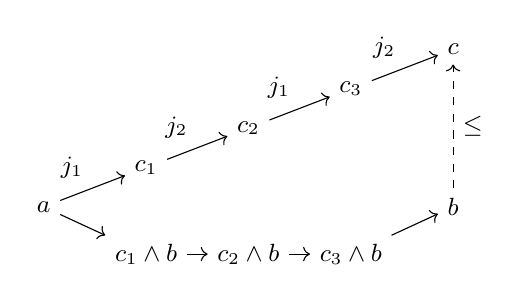
\begin{tikzpicture}[scale=1,every node/.style={font=\small}]
\node (a) at (0,0) {$a$}; \node (c1) at (1.3,0.5) {$c_1$}; \node (c2) at (2.6,1) {$c_2$};
\node (c3) at (3.9,1.5) {$c_3$}; \node (c) at (5.2,2) {$c$};
\draw[->] (a)--(c1) node[midway,above left] {$j_1$}; \draw[->] (c1)--(c2) node[midway,above left] {$j_2$};
\draw[->] (c2)--(c3) node[midway,above left] {$j_1$}; \draw[->] (c3)--(c) node[midway,above left] {$j_2$};
\node (b) at (5.2,0) {$b$};
\node (d1) at (1.3,-0.6) {$c_1\wedge b$}; \node (d2) at (2.6,-0.6) {$c_2\wedge b$}; \node (d3) at (3.9,-0.6) {$c_3\wedge b$};
\draw[->] (a)--(d1); \draw[->] (d1)--(d2); \draw[->] (d2)--(d3); \draw[->] (d3)--(b);
\draw[->,dashed] (b)--(c) node[midway,right] {$\le$};
\end{tikzpicture}
\caption{Left cancellation in Lemma~\ref{lem:chains}: an alternating chain
from $a$ to $c$ is cut down to one from $a$ to $b\le c$ by meeting with $b$;
each step keeps its index because the nuclei preserve binary meets.}
\label{fig:cut}
\end{figure}

\begin{thm}\label{thm:joins}
Let $j_1,j_2$ be nuclei preserving binary meets, $j=j_1\vee j_2$ and
$S=j_2j_1$.
\begin{enumerate}
\item[(i)] $W^L_{j_1}\vee W^L_{j_2}=W^L_j$ in $\Same(L)$ if and only if for
every $a\in L$ there is $n$ with $S^na=ja$.
\item[(ii)] $W_{j_1}\vee W_{j_2}=W_j$ in $\Same(\FSet(L))$ if and only if
there is $N$ with $S^N=j$.
\end{enumerate}
In both cases the inclusion $\subseteq$ always holds.
\end{thm}
\begin{proof}
The inclusion holds since $W_{j_1},W_{j_2}\subseteq W_j$ by monotonicity.
An alternating chain $a=c_0\le\dots\le c_n=b$ satisfies
$c_i\le j_{p(i)}c_{i-1}$; padding it with a trivial first step if it starts
with index $2$, so that the indices read $1,2,1,2,\dots$, gives
$b\le S^{\lceil(n+1)/2\rceil}a\le S^{n+1}a$. Conversely
$a\le j_1a\le j_2j_1a\le\dots\le S^na$ is an alternating chain of length $2n$.

(i) If every $a$ stabilises, let $a\le b$ with $ja=jb$. There are chains
from $a$ to $ja$ and from $b$ to $jb=ja$, so $(a\le ja)$ and $(b\le jb)$ lie
in the join by Lemma~\ref{lem:chains}, and $(a\le b)$ does by
cancellation. Conversely, $(a\le ja)\in W^L_j$; if it lies in the join there
is an alternating chain from $a$ to $ja$ of some length $n$, so
$ja\le S^{n+1}a\le ja$.

(ii) If $S^N=j$, every pair $a\le ja$ has a chain of length $2N$, and for a
bijection $f$ with $j\mu=j\nu f$ the pairs $(\mu(x)\le j\mu(x))$ and
$(\nu(fx)\le j\nu(fx))$ are uniformly chained, so $f$ is in the join by
Lemma~\ref{lem:chains} and cancellation, which preserves bounds. Conversely
suppose no $N$ works: for every $k$ there is $a_k$ with $S^{k+1}a_k\ne ja_k$,
so every alternating chain from $a_k$ to $ja_k$ has length $>k$ by the
first paragraph. Let $X=\mathbb N$, $\mu(k)=a_k$, $\nu(k)=ja_k$. The identity
$(X,\mu)\to(X,\nu)$ lies in $W_j$ but is not uniformly chained, so it is
not in $W_{j_1}\vee W_{j_2}$.
\end{proof}

\begin{cor}\label{cor:axiom}
For nuclei preserving binary meets, $W_{j_1\vee j_2}=W_{j_1}\vee W_{j_2}$ in
$\Same(\FSet(L))$ if and only if the algebra $(L,j_1,j_2,j_1\vee j_2)$
validates the finite-iteration axiom $(\laxb\laxa)^N\varphi\leftrightarrow
\lax\varphi$ of $\LLJ$ for some $N$ \cite{Laxjoin}. In particular this holds
for every finite $L$, for $L=\Up(P)$ with $P$ a finite poset ($N=|P|$),
and whenever $\Nuc(L)$ satisfies the ascending chain condition on
$\{S^n:n\in\mathbb N\}$.
\end{cor}

\begin{rem}
The join of samenesses is computed by chains of \emph{bounded} length and
the join of nuclei by transfinite iteration; Theorem~\ref{thm:joins} is the
statement that the two agree exactly when the iteration is uniformly
finite. This is the mechanism of \cite{Topjoin,Finitejoin} for Grothendieck
topologies, where the alternating products of two idempotent ideals must
stabilise, reduced to its degreewise core: the category of fuzzy sets has
no gluing, so nothing but the arithmetic of $L$ is involved, and the
pointwise condition of (i) is the residue of (ii) on a single point.
\end{rem}

\section{The standard algebras}\label{sec:std}

\begin{prop}\label{prop:mv}
Let $A$ be a complete MV-algebra. Then every nucleus on $A$ is closed,
$j(a)=a\vee c$ with $c=j(\bot)$, and $c\mapsto(-)\vee c$ is a lattice
isomorphism $A\cong\Nuc(A)$. Consequently $j_2j_1=j_1\vee j_2$ for all
nuclei, and $c\mapsto W_{(-)\vee c}$ is a lattice embedding
$A\hookrightarrow\Same(\FSet(A))$ and $A\hookrightarrow\Same(A)$, where
$W_{(-)\vee c}$ is the class of bijections $f$ with
$\mu\vee c=(\nu\circ f)\vee c$.
\end{prop}
\begin{proof}
Let $j$ be a nucleus and $b\in\Fix(j)$. Then $a\to b\in\Fix(j)$ for every
$a$. In an MV-algebra $a\to b=\neg a\oplus b$, and for every $x\ge b$ we have
$b\oplus(x\otimes\neg b)=b\vee x=x$, so $x=a\to b$ for $a=\neg(x\otimes\neg
b)$; hence $\uparrow\!b\subseteq\Fix(j)$. So $\Fix(j)$ is an up-set closed
under meets, i.e.\ $\Fix(j)=\uparrow\!c$ with $c=\bigwedge\Fix(j)=j(\bot)$,
and $j(a)=a\vee c$. Conversely $a\mapsto a\vee c$ is a nucleus:
$(a\vee c)\otimes(b\vee c)=(a\otimes b)\vee(a\otimes c)\vee(c\otimes b)\vee
(c\otimes c)\le(a\otimes b)\vee c$ by integrality. The map $c\mapsto(-)\vee c$
is an order isomorphism $A\to\Nuc(A)$, with
$\Fix((-)\vee c)\cap\Fix((-)\vee d)=\uparrow\!(c\vee d)$ and pointwise meet
$(-)\vee(c\wedge d)$ by distributivity. For the iteration, $j_2j_1a=a\vee c
\vee d$ is already fixed by both. Closed nuclei on a distributive lattice
preserve binary meets, so Theorems~\ref{thm:meets} and~\ref{thm:joins}
apply with $N=1$, and injectivity is Theorem~\ref{thm:meets}.
\end{proof}

\begin{prop}\label{prop:product}
On the product chain $[0,1]_\Pi$ ($a\otimes b=ab$, $a\to b=\min(1,b/a)$ for
$a>0$, $0\to b=1$) the nuclei are exactly the closed nuclei
$p_c(a)=a\vee c$, $c\in[0,1]$, and the maps $q_c$, $c\in(0,1]$, with
$q_c(0)=0$ and $q_c(a)=a\vee c$ for $a>0$. All of them preserve binary
meets, $(j_2j_1)^2=j_1\vee j_2$ for any two of them, and $j\mapsto W_j$ is a
lattice embedding $\Nuc([0,1]_\Pi)\hookrightarrow\Same(\FSet([0,1]_\Pi))$.
\end{prop}
\begin{proof}
Let $j$ be a nucleus. If $b>0$ is fixed then so is $a\to b=b/a$ for
$a\in[b,1]$, which runs through $[b,1]$; so $\Fix(j)\cap(0,1]$ is an
up-set of $(0,1]$ closed under infima, hence $(0,1]$, $[c,1]$ with $c>0$,
or (as $1$ is fixed) never empty. The value $0$ is fixed or not, and
$a\to0\in\{0,1\}$ imposes nothing. If $\Fix(j)\cap(0,1]=(0,1]$ then $0$ is
fixed as the infimum, giving $p_0=\mathrm{id}$; otherwise $\Fix(j)=[c,1]$
or $\{0\}\cup[c,1]$ with $c>0$, giving $p_c$ or $q_c$. Conversely $p_c$ is a
nucleus as in Proposition~\ref{prop:mv}, and $q_c$ is one: $q_c(a)q_c(b)=0
\le q_c(ab)$ if $a=0$ or $b=0$, and otherwise $(a\vee c)(b\vee c)=\max(ab,ac,
cb,c^2)\le\max(ab,c)=q_c(ab)$. Both kinds preserve binary meets, the
chain being distributive and $q_c$ agreeing with $p_c$ on $(0,1]$ and
fixing $0$. For the iteration, on $a>0$ every composite of two of these
nuclei is $a\vee c\vee d$, fixed by both; at $0$ the only nontrivial case is
$j_1=q_c$, $j_2=p_d$ with $d>0$, where $j_2j_1(0)=d$ and
$(j_2j_1)^2(0)=d\vee c=(j_1\vee j_2)(0)$, as $\Fix(q_c)\cap\Fix(p_d)=[c\vee d,1]$.
So $N=2$ always works and Theorem~\ref{thm:joins} gives the embedding, with
Theorem~\ref{thm:meets} for meets and injectivity. Note that
$\Nuc([0,1]_\Pi)$ is not isomorphic to $[0,1]$: it is the chain of the $p_c$
with a second copy $q_c<p_c$ of its positive part attached.
\end{proof}

\begin{rem}
In the language of \cite{Laxjoin}, the lax modalities of \L ukasiewicz logic
with truth constants are the disjunctions $\lax\varphi=\varphi\vee c$, and
the join of two of them is the disjunction with $c\vee d$: the trimodal
logic $\LLJ$ over \L ukasiewicz logic collapses to its finite-iteration
instance with $N=1$. Over G\"odel logic, where nuclei are the Heyting ones,
no such collapse occurs, as the next examples show.
\end{rem}

\begin{ex}\label{ex:godel}
Let $L=[0,1]$ with the G\"odel operations, $\otimes=\min$ and $a\to b=1$ if
$a\le b$, $=b$ otherwise. Since $\{a\to b:a\in L\}=\{b,1\}$, the fixed-point
sets of nuclei are exactly the subsets $F\ni1$ closed under infima, with
$j_F(a)=\min\{f\in F:f\ge a\}$; all nuclei preserve binary meets.
\begin{enumerate}
\item[(a)] \emph{Pointwise but not uniformly.} Let
$F_1=\{0,1\}\cup\{1/(2k):k\ge1\}$ and $F_2=\{0,1\}\cup\{1/(2k+1):k\ge1\}$,
both inf-closed. Then $\Fix(j_1\vee j_2)=F_1\cap F_2=\{0,1\}$, so $j(0)=0$
and $j(a)=1$ for $a>0$. From $a=1/n$ the alternating iteration moves
$1/n\mapsto1/(n-1)\mapsto\cdots\mapsto1$, with $n-1$ nontrivial steps (the
first step is trivial when $1/n\in F_1$), and $0$ is fixed;
so every point stabilises but no $N$ works. By Theorem~\ref{thm:joins},
$W^L_{j_1}\vee W^L_{j_2}=W^L_j$ in $\Same([0,1]_G)$ while $W_{j_1}\vee W_{j_2}
\subsetneq W_j$ in $\Same(\FSet([0,1]_G))$: the identity
$(\mathbb N,n\mapsto1/n)\to(\mathbb N,n\mapsto1)$ is an isomorphism up to
$j$ but not a bounded alternation of isomorphisms up to $j_1$ and up to $j_2$.
\item[(b)] \emph{Not even pointwise.} Let $F_1=\{1\}\cup\{1-1/(2k):k\ge1\}$
and $F_2=\{1\}\cup\{1-1/(2k+1):k\ge1\}$. Then $F_1\cap F_2=\{1\}$, so
$j$ is the constant $1$, while the iteration from $0$ runs through
$1/2,2/3,3/4,\dots$ and never reaches $1$. Hence $(0\le1)\in W^L_j$ is in
neither join: $W^L_{j_1}\vee W^L_{j_2}\subsetneq W^L_j$ already in
$\Same([0,1]_G)$. This is the G\"odel-chain form of the inexpressibility
example of \cite[\S5]{Laxjoin}.
\end{enumerate}
\end{ex}

\begin{figure}[ht]
\centering
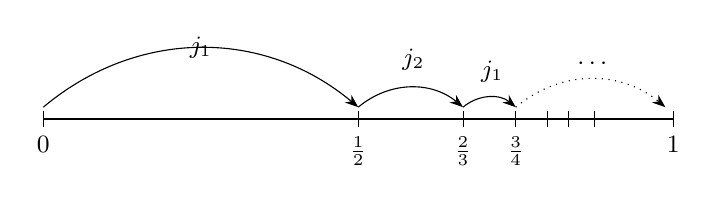
\begin{tikzpicture}[scale=1,every node/.style={font=\small}]
\draw[thick] (0,0)--(8,0);
\foreach \x/\l in {0/$0$,8/$1$} {\draw (\x,-0.1)--(\x,0.1); \node[below] at (\x,-0.1) {\l};}
\foreach \k in {2,3,4,5,6,8} {\pgfmathsetmacro{\x}{8*(1-1/\k)} \draw (\x,-0.1)--(\x,0.1);}
\node[below] at (4,-0.1) {$\tfrac12$}; \node[below] at (5.33,-0.1) {$\tfrac23$}; \node[below] at (6,-0.1) {$\tfrac34$};
\draw[->,>=Stealth] (0,0.15) to[bend left=40] (4,0.15); \node at (2,0.9) {$j_1$};
\draw[->,>=Stealth] (4,0.15) to[bend left=40] (5.33,0.15); \node at (4.7,0.75) {$j_2$};
\draw[->,>=Stealth] (5.33,0.15) to[bend left=40] (6,0.15); \node at (5.7,0.6) {$j_1$};
\draw[->,>=Stealth,dotted] (6,0.15) to[bend left=40] (7.9,0.15);
\node at (7,0.7) {$\cdots$};
\end{tikzpicture}
\caption{Example~\ref{ex:godel}(b) on the G\"odel chain $[0,1]$: the
alternating iteration from $0$ climbs $1-1/k$ and never reaches
$(j_1\vee j_2)(0)=1$.}
\label{fig:godel}
\end{figure}

\begin{ex}
For $L=\Up(P)$, the up-sets of a poset, the nuclei $\lax_CU=\{x:\uparrow\!x
\cap C\subseteq U\}$ of \cite{Laxjoin,Relnec} preserve binary meets. For
finite $P$ every nucleus is of this form and $(j_2j_1)^{|P|}=j_1\vee j_2$
\cite[Thm.~4.1]{Laxjoin}, so $\Nuc(\Up(P))\cong(\mathcal P(P),\supseteq)$
embeds as a lattice into $\Same(\FSet(\Up(P)))$. For infinite $P$ the join
$\lax_C\vee\lax_{C'}$ equals $\lax_{C\cap C'}$ iff $P$ has no $(C\cap C')$-free
alternating chain \cite{Relnec}, a different condition from the
stabilisation of the iteration; Example~\ref{ex:godel}(a) and (b) are modelled on
$\Up(\omega+1)$ and $\Up(\omega+2)$ with the even and odd points, whose
up-sets form chains.
\end{ex}

\section{Remarks on the logical reading}\label{sec:logic}

A triple $(L,j_1,j_2,j_1\vee j_2)$ is an algebra of the lax logic $\LLJ$
of two nuclei and their join \cite{Laxjoin}, and fuzzy sets over $L$ are its
natural models: a fuzzy set $(X,\mu)$ assigns to each point a degree, the
modalities act on degrees, and $W_j$ consists of the maps along which the
$j$-modalised degrees are transported isomorphically. Theorem~\ref{thm:joins}
then reads: the isomorphisms up to the join modality are generated, by
composition and two-out-of-three, by the isomorphisms up to the two
modalities if and only if the join modality is a finite iterate of the two,
the finite-iteration axiom. Over \L ukasiewicz logic the axiom holds with
$N=1$ and the modalities are disjunctions with constants
(Proposition~\ref{prop:mv}), over product logic with $N=2$
(Proposition~\ref{prop:product}); over G\"odel logic it may fail
(Example~\ref{ex:godel}). The other operations of $\FSet(L)$, in particular
the $\alpha$-cuts $X_\alpha=\{x:\mu(x)\ge\alpha\}$, give samenesses
$W_\alpha=\{f:f\text{ restricts to a bijection }X_\alpha\to Y_\alpha\}$ that
are not of the form $W_j$ and do not preserve joins of levels
($W_\alpha\cap W_\beta\not\subseteq W_{\alpha\vee\beta}$ on $L=\mathbf 2\times
\mathbf 2$); the structure of $\Same(\FSet(L))$ beyond the image of
$\Nuc(L)$ is left open.

\begin{que}
For which $L$ is every element of $\Same(\FSet(L))$ contained in $\Bij$
generated by the classes $W_j$ and the cut classes $W_\alpha$? Does
Theorem~\ref{thm:joins}(ii) extend to nuclei that do not preserve binary
meets?
\end{que}

\section*{Funding}
No funding was received for this work.

\section*{Declarations}
The author has no competing interests to declare.

\begin{thebibliography}{9}
\bibitem{Barr} M.~Barr, \emph{Fuzzy set theory and topos theory}, Canad.
Math. Bull. \textbf{29} (1986), 501--508.
\bibitem{BCD} S.~Buss, D.~Casta\~no, J.~P.~D\'\i az Varela, \emph{Terms that
define nuclei on residuated lattices: a case study of BL-algebras}, preprint,
arXiv:2412.19690, 2024.
\bibitem{Escardo} M.~H.~Escard\'o, \emph{Joins in the frame of nuclei}, Appl.
Categ. Structures \textbf{11} (2003), 117--124.
\bibitem{FM} M.~Fairtlough, M.~Mendler, \emph{Propositional lax logic},
Inform. and Comput. \textbf{137} (1997), 1--33.
\bibitem{GJKO} N.~Galatos, P.~Jipsen, T.~Kowalski, H.~Ono, \emph{Residuated
Lattices: An Algebraic Glimpse at Substructural Logics}, Elsevier, 2007.
\bibitem{Goguen} J.~A.~Goguen, \emph{$L$-fuzzy sets}, J. Math. Anal. Appl.
\textbf{18} (1967), 145--174.
\bibitem{Hajek} P.~H\'ajek, \emph{Metamathematics of Fuzzy Logic}, Kluwer,
1998.
\bibitem{Johnstone} P.~T.~Johnstone, \emph{Stone Spaces}, Cambridge University
Press, 1982.
\bibitem{Macnab} D.~S.~Macnab, \emph{Modal operators on Heyting algebras},
Algebra Universalis \textbf{12} (1981), 5--29.
\bibitem{Rosenthal} K.~I.~Rosenthal, \emph{Quantales and Their Applications},
Longman, 1990.
\bibitem{Same} R.~Shibusawa, \emph{The sameness lattice of a category:
weak-equivalence structures, Galois functoriality, and comparison intervals},
preprint, 2026, DOI 10.5281/zenodo.22823772.
\bibitem{Topjoin} R.~Shibusawa, \emph{Meets and joins of Grothendieck
topologies in the sameness lattice}, preprint, 2026, DOI 10.5281/zenodo.22978446.
\bibitem{Finitejoin} R.~Shibusawa, \emph{Grothendieck topologies on a finite
category form a sublattice of the lattice of two-out-of-three classes},
preprint, 2026, DOI 10.5281/zenodo.23204943.
\bibitem{Varieties} R.~Shibusawa, \emph{Lattices of subvarieties and of
logics as sublattices of the lattice of two-out-of-three classes}, preprint,
2026, DOI 10.5281/zenodo.23407364.
\bibitem{Laxjoin} R.~Shibusawa, \emph{The join of two nuclei as a lax modality:
axiomatization, finite models, and inexpressibility}, preprint, 2026,
DOI 10.5281/zenodo.23330576.
\bibitem{Relnec} R.~Shibusawa, \emph{Joins of relativized necessities on a
poset: an alternating-chain criterion and the induction scheme of lax
logic}, preprint, 2026, DOI 10.5281/zenodo.23411203.
\end{thebibliography}

\end{document}
